%\newcommand{\CLASSINPUTrighttextmargin}{0.62cm}
\documentclass[conference]{IEEEtran}
\IEEEoverridecommandlockouts
\usepackage{cite}
\usepackage{float}
\usepackage{amsmath,amssymb,amsfonts}
\usepackage{graphicx}
\usepackage{tikz}
\usetikzlibrary{arrows.meta, positioning}
\usepackage{textcomp}
\usepackage{xcolor}
\usepackage{multirow}
\usepackage{scalefnt}
\usepackage{booktabs}
\usepackage{url}
\usepackage[brazil]{babel}
\usepackage{siunitx}
\sisetup{output-decimal-marker={,}, group-separator={.}}
\usepackage{listings}
\lstset{
  basicstyle=\ttfamily\footnotesize,
  breaklines=true,
  frame=single,
  language=Python,
  showstringspaces=false,
  columns=fullflexible
}
\graphicspath{{figuras/}}

\begin{document}

\title{Processamento Digital de Sinais: Filtros de Butterworth, Chebyshev e Elíptico}

\author{Aruan Bretas de Oliveira Filho, Isabela Muller Martins Rocha, João Marcelo Trovão Filho e Murilo Vinicius da Silva
\thanks{Projeto Final da disciplina SEL0615 (Processamento Digital de Sinais), Escola de Engenharia de São Carlos, Universidade de São Paulo. Grupo B9.}}

\maketitle

\section{Fundamentação Teórica}

No presente trabalho, valeu-se de filtros IIR para resolução de uma situação problema que exigia a minimização de ruído em um sinal dado, com frequência fundamental de 60hz. Para tanto, valemo-nos de diferentes modelos (a saber, Butterworth, Chebyshev tipo I e II, e Elíptico), alterando os parâmetros julgados relevantes de modo a minimizar o erro frente ao sinal original, ponderando pelo impacto computacional que a solução traria.

Em relação aos algoritmos avaliados, temos também particularidades teóricas em seu funcionamento, conforme explicitado em \cite{oppenheim2009} que podem explicar a adequação (ou não) à situação presente. Em comum, todos são filtros digitais passa baixa, atuando de modo a retirar as frequências indesejadas introduzidas no ruído. No entanto, há divergências de funcionamento, particularmente em relação à velocidade e suavidade de transição nas diferentes bandas do sinal, e consequentemente no ripple acarretado.

Para o filtro Butterworth, temos que sua resposta em magnitude é monotônica, tanto na banda de aceitação quanto de corte, ou seja, não introduz ripple, sendo uma opção de filtro bem suave. Conforme aumentamos a ordem, no entanto, é observado um comportamento mais brusco de transição

Já os filtros de Chebyshev aceitam a existência de ripple, mas apenas em uma das bandas, seja na de aceitação , mantendo a banda de rejeição monotônica (tipo I); Ou na de rejeição, mantendo a banda de aceitação plana (tipo II). Apesar de indesejado, a introdução do ripple pode ser útil visto que tem como consequência uma transição consideravelmente mais rápida que filtros monotônicos, como Butterworth

Por fim, o filtro Elíptico permite existência de ripple em todo seu espectro, tanto na banda de aceitação quanto de rejeição. Isso torna sua transição bem agressiva, possuindo a faixa de transição mais rápida de todos, mas ocasionando em um erro distribuído maior.


\begin{figure}[h]
\centering
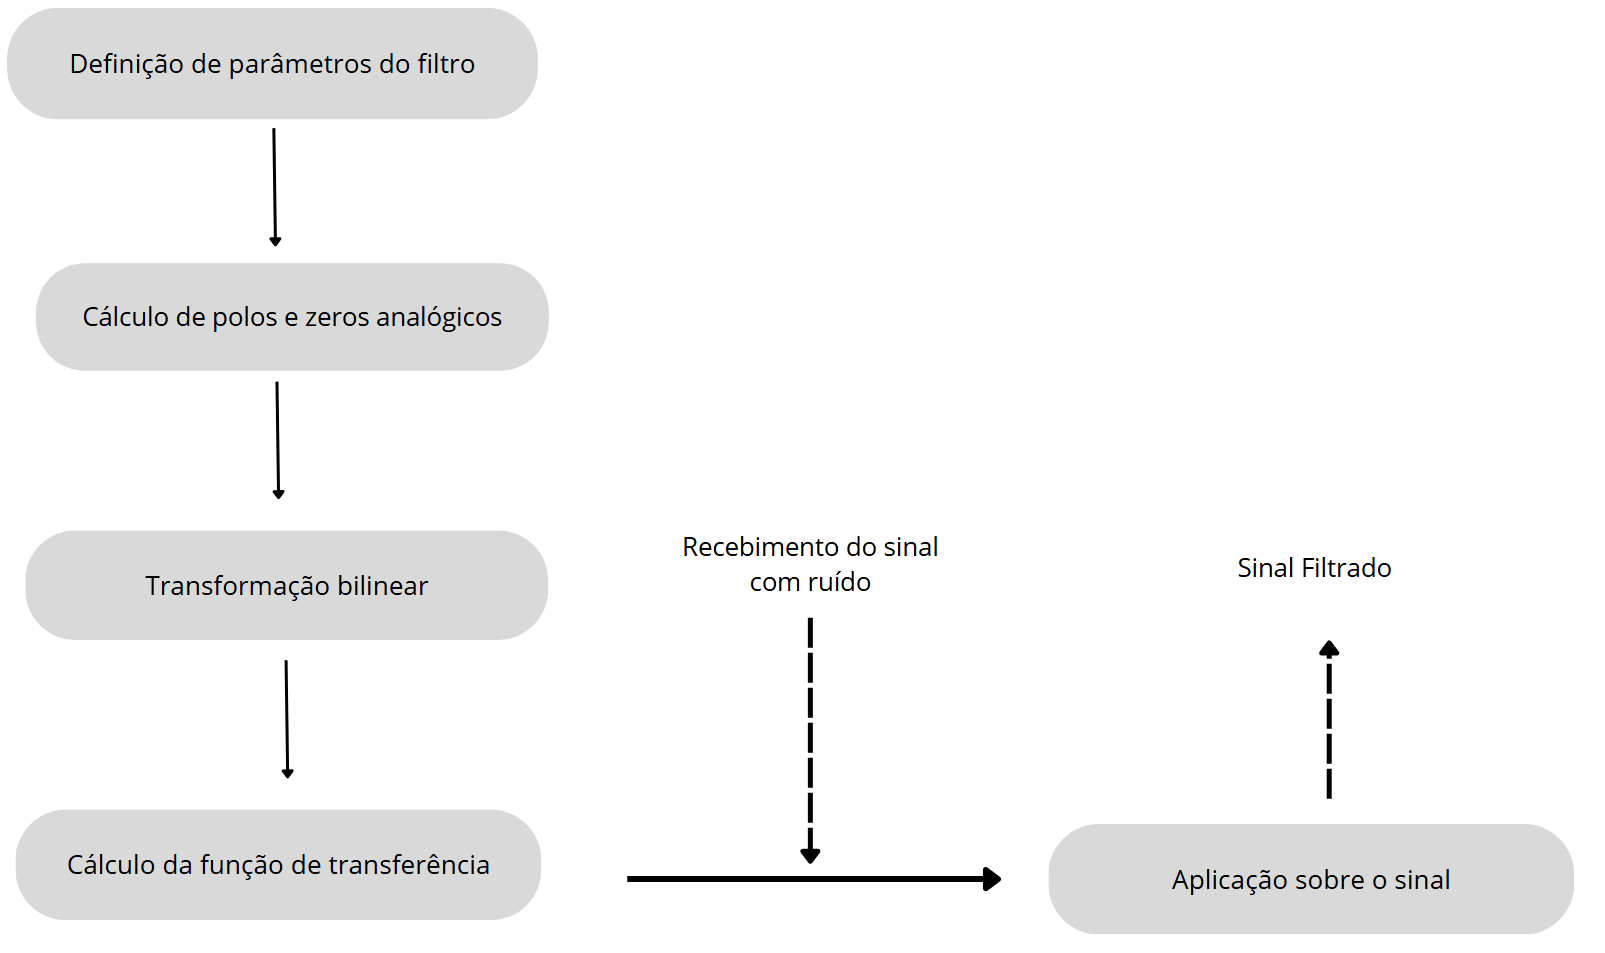
\includegraphics[width=0.45\textwidth]{Fluxograma.png}
\caption{Fluxograma do filtro de Chebyshev Tipo II}
\label{fig:flowchart}
\end{figure}

\subsection{Filtros IIR e Transformação Bilinear}
Um filtro IIR é descrito por uma equação de diferenças recursiva~\cite{oppenheim2009},
cuja função de transferência no domínio~$z$ é uma razão de polinômios:
\begin{equation}
H(z) = \frac{\sum_{k=0}^{M} b_k\,z^{-k}}{1 + \sum_{k=1}^{N} a_k\,z^{-k}}.
\label{eq:Hz}
\end{equation}
A recursividade (presença de polos) permite obter respostas seletivas com ordens
baixas, ao custo de exigir verificação de estabilidade: todos os polos devem
estar no interior do círculo unitário, $|p_i| < 1$. O projeto parte de um
protótipo analógico passa-baixas, mapeado para o domínio discreto pela
\emph{transformação bilinear}
\begin{equation}
s = \frac{2}{T}\,\frac{1 - z^{-1}}{1 + z^{-1}},
\end{equation}
que preserva a estabilidade, mas introduz distorção de frequência
(\emph{warping}), compensada por pré-distorção (\emph{prewarping}) na frequência
de corte. As rotinas utilizadas executam esse procedimento internamente.

\subsection{Filtragem Causal versus Fase Zero}
A filtragem direta (\emph{causal}) introduz atraso de fase dependente da
frequência, deformando a forma de onda. Em processamento \emph{offline}, a
filtragem de \textbf{fase zero} aplica o filtro duas vezes, nos sentidos direto e
reverso, cancelando o atraso de fase e dobrando a atenuação efetiva~\cite{gustafsson}.
Ambas as estratégias foram avaliadas: a causal por funcionar em tempo real e a de
fase zero por ter melhor desempenho \emph{offline}.

\subsection{Realização em Seções de Segunda Ordem (SOS)}
Para ordens elevadas, a forma direta~\eqref{eq:Hz} é numericamente mal
condicionada: o erro de arredondamento dos coeficientes pode levar à
instabilidade. Por isso adotou-se a realização em \textbf{seções de segunda
ordem} (cascata de biquads), bem mais robusta e de uso comum na prática.

\subsection{Métricas de Avaliação}
A qualidade da filtragem é medida pelo \textbf{erro quadrático médio}
\begin{equation}
\mathrm{RMSE} = \sqrt{\frac{1}{L}\sum_{n=0}^{L-1}
\bigl(x[n] - \hat{x}[n]\bigr)^2},
\label{eq:rmse}
\end{equation}
onde $x$ é o sinal de referência e $\hat{x}$ o sinal filtrado. Complementarmente,
o \textbf{ganho de relação sinal-ruído} (SNR) quantifica a melhoria em decibéis:
\begin{equation}
\Delta\mathrm{SNR} = 10\log_{10}\!\frac{\sum x^2}{\sum (\hat{x}-x)^2}
                   - 10\log_{10}\!\frac{\sum x^2}{\sum (x_{\text{ruído}}-x)^2}.
\label{eq:snr}
\end{equation}

\subsection{Implementação da Função de Filtragem}
A filtragem foi implementada em Python (bibliotecas \texttt{numpy} e
\texttt{scipy.signal}~\cite{scipy}) como uma função genérica, aplicável a qualquer
comprimento de sinal:

\begin{lstlisting}
def aplicar_filtro_iir(sinal, fs, f_corte, ordem,
                       tipo='butter', rp=0.5, rs=40.0,
                       fase_zero=True):
    Wn = f_corte / (0.5 * fs)
    sos = projetar_sos(tipo, ordem, Wn, rp, rs)
    if fase_zero:
        return signal.sosfiltfilt(sos, sinal), sos
    return signal.sosfilt(sos, sinal), sos
\end{lstlisting}

O projeto retorna os coeficientes em formato SOS; a filtragem de fase zero usa
\texttt{sosfiltfilt} e a causal, \texttt{sosfilt}. A frequência de corte é
normalizada pela frequência de Nyquist ($f_s/2$). Cabe ressaltar que o
significado de $f_c$ depende da aproximação: no Butterworth corresponde ao ponto
de \SI{-3}{\decibel}; no Chebyshev~I e no elíptico, à borda da banda de passagem
(onde termina a ondulação $r_p$); e no Chebyshev~II, à borda da banda de
\emph{rejeição} (onde a atenuação atinge $r_s$). Assim, o valor
$f_c=\SI{2700}{\hertz}$ do Chebyshev~II selecionado marca o início da banda de
rejeição, com a banda de passagem efetiva situada em frequência inferior.

\subsection{Busca em Grade e Critério de Estabilidade}
Para determinar os parâmetros ótimos, varreu-se uma grade de
\begin{itemize}
  \item \textbf{tipo}: \{Butterworth, Chebyshev~I, Chebyshev~II, elíptico\};
  \item \textbf{ordem}: de~1 a~8;
  \item \textbf{frequência de corte}: de \SI{300}{\hertz} a \SI{3300}{\hertz},
        em passos de \SI{100}{\hertz};
  \item \textbf{ondulação de passagem} $r_p$ (Chebyshev~I e elíptico):
        \{0{,}1;\ 0{,}5;\ 1{,}0\}~dB;
  \item \textbf{atenuação de rejeição} $r_s$ (Chebyshev~II e elíptico):
        \{30;\ 40;\ 50;\ 60\}~dB;
  \item \textbf{método}: fase zero e causal.
\end{itemize}
Vale uma observação sobre o enunciado, que pede testar diferentes
\emph{ordens} e \emph{janelamentos}. O janelamento é um parâmetro de projeto de
filtros FIR (resposta finita ao impulso), em que a resposta ao impulso
é truncada por uma janela como Hamming, Hann ou Kaiser; em filtros IIR ele não se
aplica, porque o filtro vem de um protótipo analógico mapeado para o
domínio discreto. O
parâmetro equivalente, que molda o formato da resposta, é o par
ondulação/atenuação ($r_p$, $r_s$); por isso a grade o varre
junto com tipo, ordem e frequência de corte.

Cada configuração foi submetida a uma verificação de estabilidade (todos os
polos com $|p_i|<1$, obtidos de \texttt{sos2zpk}). Como o projeto parte de
protótipos analógicos mapeados pela transformação bilinear, que preserva a
estabilidade, todas as \num{9920} configurações da grade resultaram estáveis;
elas foram então ordenadas pelo RMSE da Eq.~\eqref{eq:rmse}.

\subsection{Avaliação do Custo Computacional}
O custo foi medido cronometrando o processo completo (projeto dos
coeficientes mais filtragem) e tomando a \textbf{mediana} de \num{50}
execuções, o que reduz a influência das variações do sistema operacional. Depois
variou-se a ordem do filtro, com tipo e corte fixos, para ver o
compromisso entre RMSE e tempo de execução.


% !TEX root = ProjetoPDS.tex
\section{Análise dos Sinais}

\subsection{Caracterização do Sinal}
\begin{figure}[H]
\centering
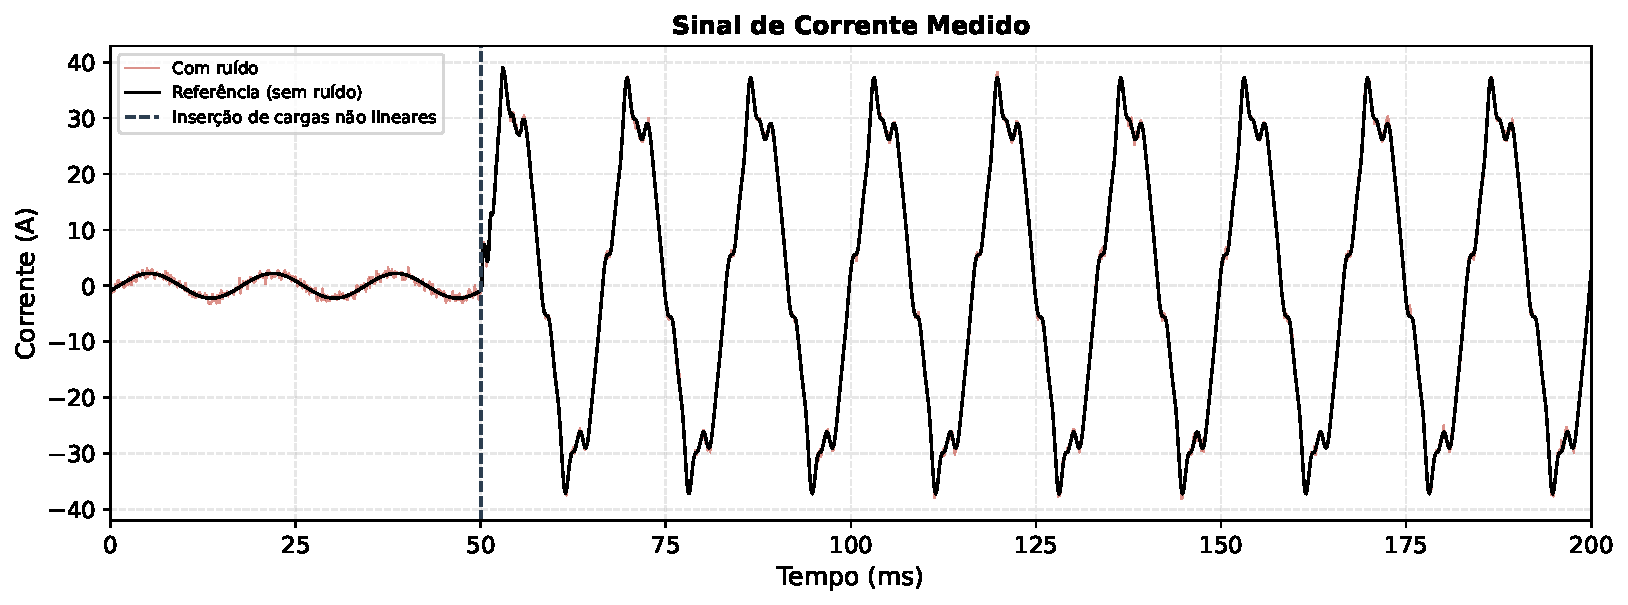
\includegraphics[width=\columnwidth]{sinal_bruto_b9.pdf}
\caption{Sinal de corrente medido (registro ruidoso e referência sem ruído), com
o instante de inserção das cargas não lineares destacado.}
\label{fig:sinal}
\end{figure}

O sinal possui \num{1537} amostras (\SI{0.20}{\second} a \SI{7680}{\hertz}) e
está reproduzido na Fig.~\ref{fig:sinal}, que mostra o registro ruidoso, a
referência sem ruído e o instante de inserção das cargas não lineares. Esse
instante foi localizado na amostra~384 ($t \approx \SI{50}{\milli\second}$) por um
detector de degrau da envoltória: calcula-se o valor eficaz (RMS) ciclo a ciclo da
fundamental (\num{128} amostras) e toma-se a maior variação entre ciclos
consecutivos. Nessa fronteira o RMS salta de \SI{1.57}{\ampere}, sob cargas
lineares, para \SI{23.1}{\ampere} após o chaveamento, confirmando a transição; a
filtragem proposta preserva esse transitório.

Distinguem-se dois regimes de operação. Antes do chaveamento, com cargas
lineares, a corrente é quase senoidal e de baixa amplitude (poucos ampères).
Depois da entrada das cargas não lineares, a amplitude cresce de repente
(fundamental de \SI{32.3}{\ampere}) e a forma de onda deixa de ser senoidal,
achatada pelos harmônicos de ordem $6k\pm1$. O desafio da filtragem é duplo: tirar
o ruído de medição, de banda larga, sem suavizar a distorção harmônica do segundo
regime, que é justamente a informação útil para a análise de qualidade de energia.

\subsection{Filtragem no Domínio do Tempo}
\begin{figure*}[t]
\centering
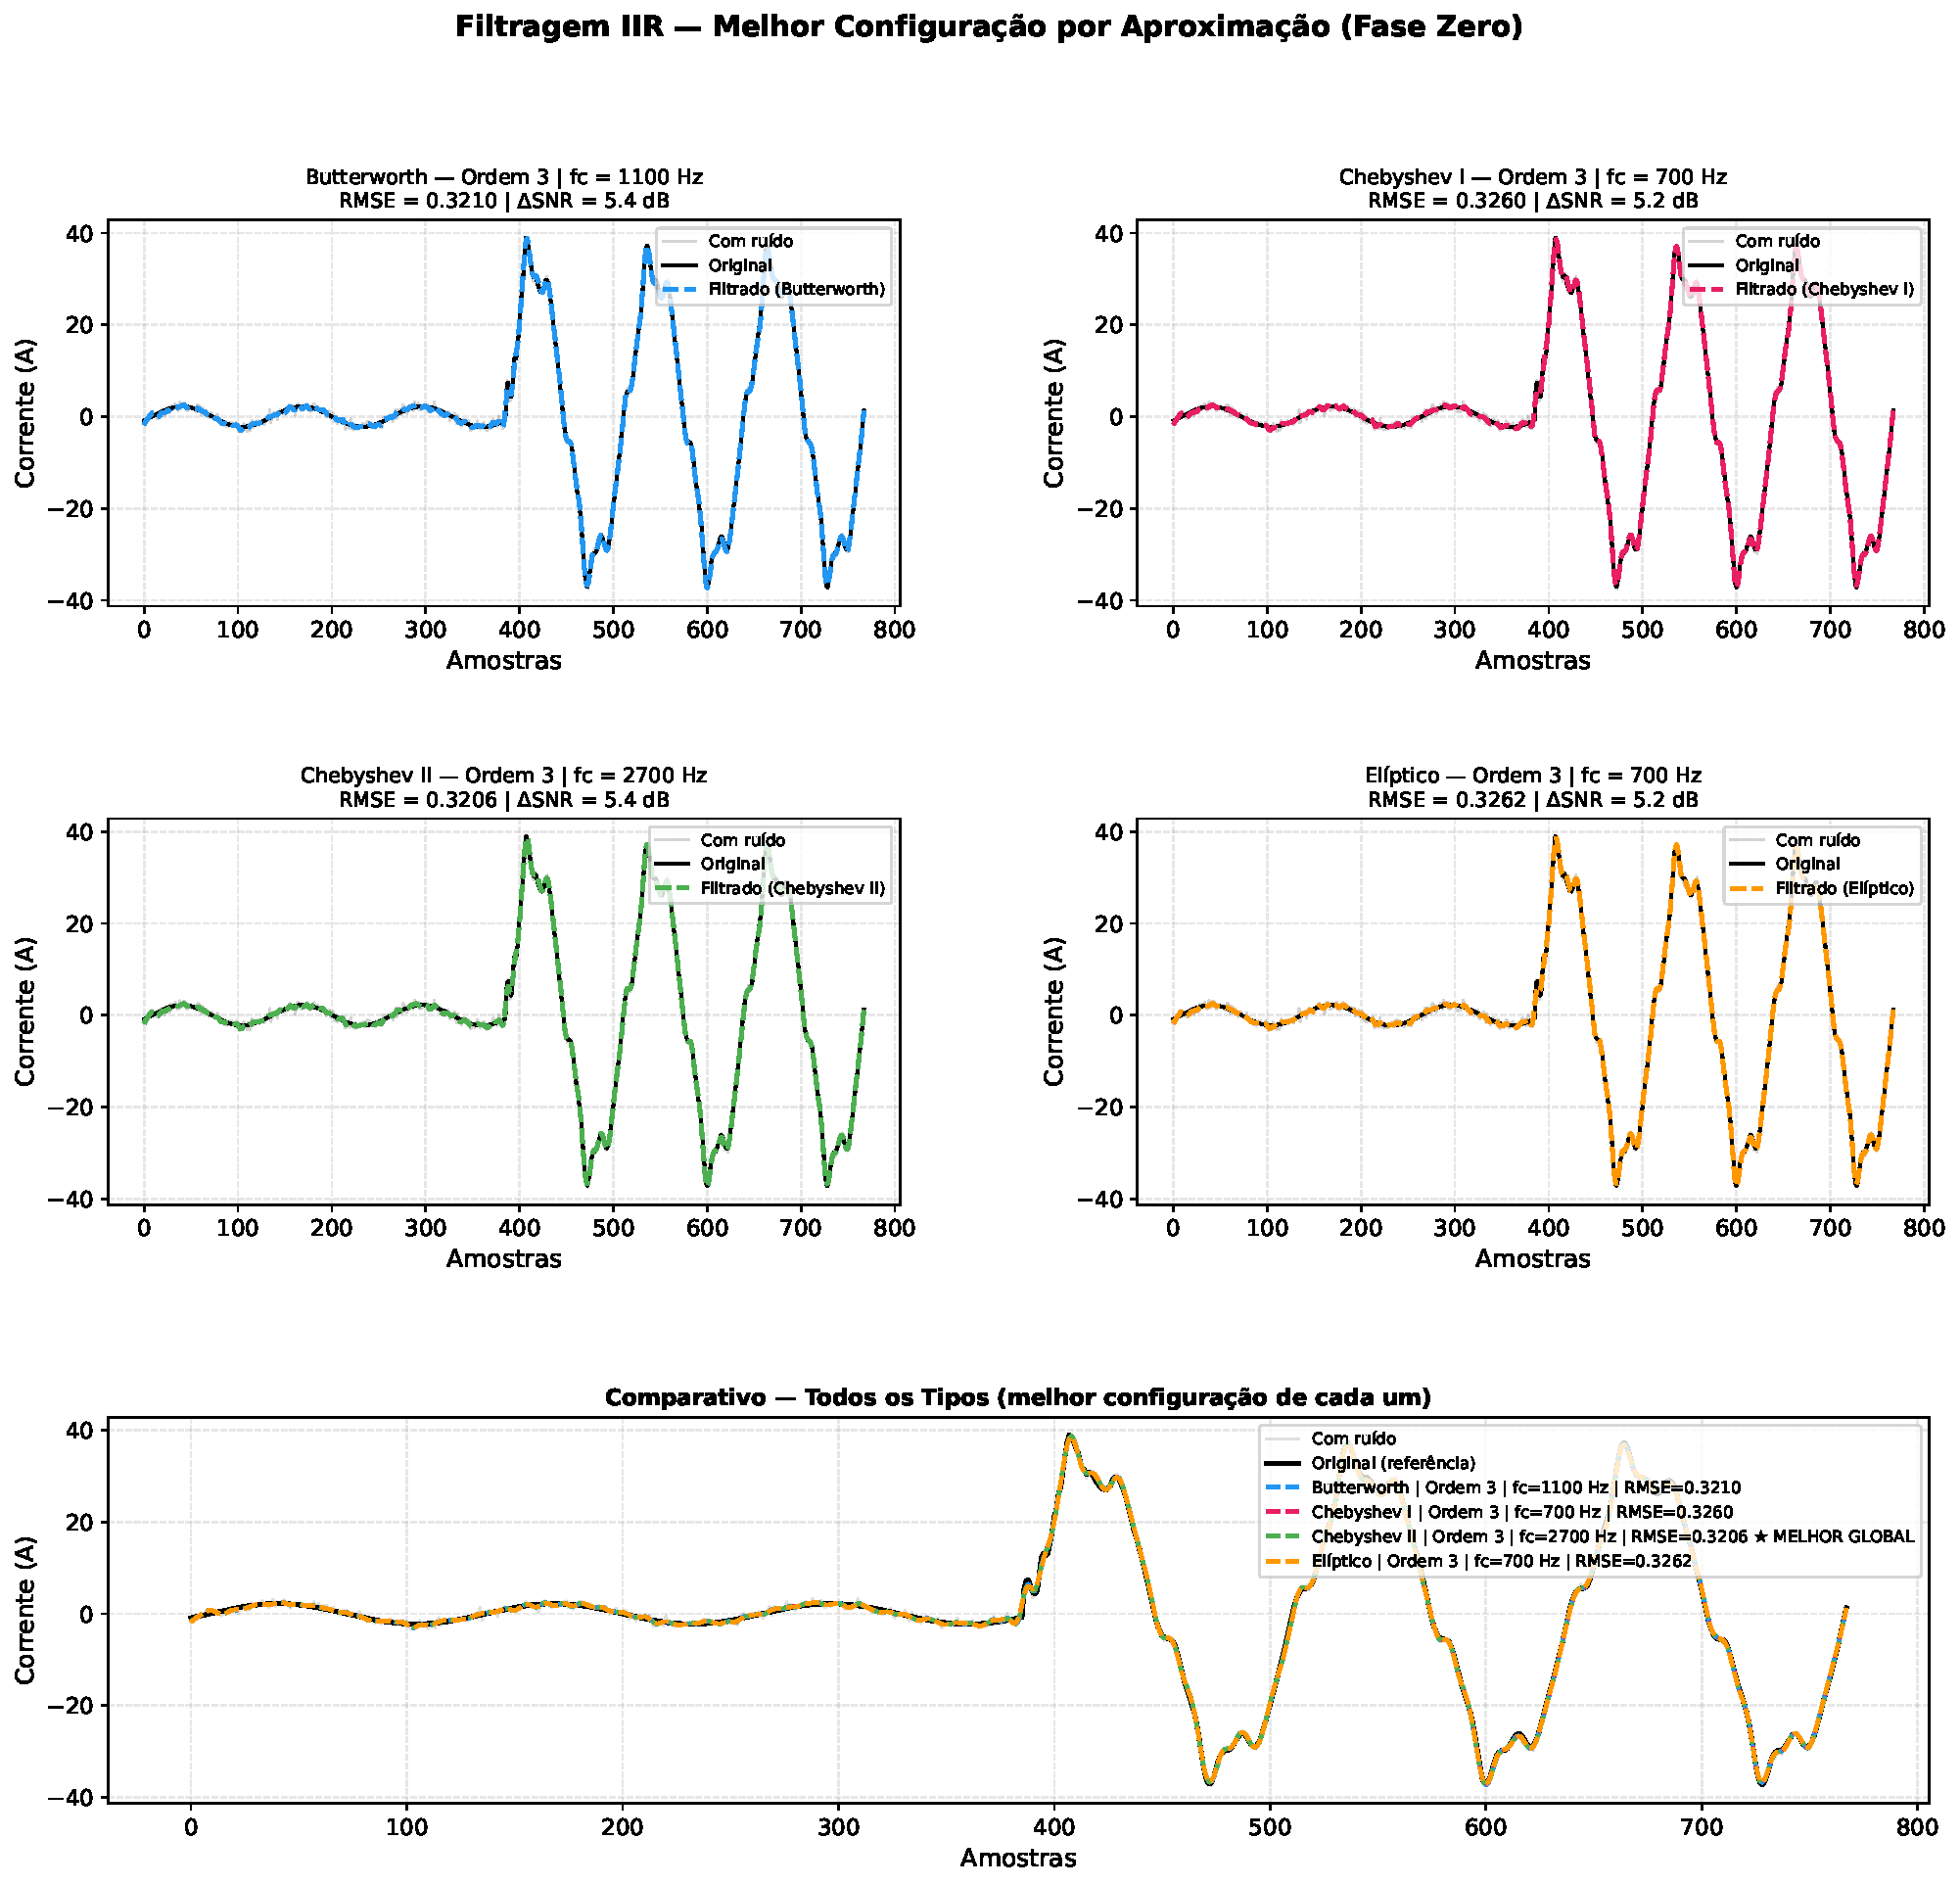
\includegraphics[width=0.92\textwidth]{resultado_filtros_iir_b9.pdf}
\caption{Filtragem no domínio do tempo: a melhor configuração de cada aproximação
sobre os sinais de referência e ruidoso (painéis superiores) e o erro residual
(filtrado menos referência) das quatro aproximações, sobreposto e ampliado no
transitório do chaveamento (painel inferior), fase zero.}
\label{fig:tempo}
\end{figure*}

A Fig.~\ref{fig:tempo} traz, nos quatro painéis superiores, o melhor filtro de cada
aproximação sobre os sinais de referência e ruidoso; na escala cheia as três curvas
ficam quase coincidentes --- efeito da filtragem eficaz e do ruído pequeno frente ao
sinal ---, evidenciando que o ruído é removido e a forma de onda preservada nos dois
regimes. O painel inferior amplia o \emph{erro residual} (filtrado menos referência)
das quatro aproximações na janela do chaveamento (amostras~300--460) --- a grandeza
minimizada pelo RMSE ---, justamente onde elas mais se distinguem: os filtros de
corte mais baixo (Chebyshev~I e elíptico, fc~$=700$~Hz) apresentam o maior
sobressinal e oscilação após o degrau --- passa-banda estreita implica resposta ao
impulso mais longa ---, enquanto o Chebyshev~II ($\star$, fc~$=2700$~Hz) reage de
forma mais contida, o que se reflete no seu menor RMSE. Fora desse transitório o erro
é pequeno (décimos de ampère) e semelhante nas quatro.

\subsection{Funções de Transferência e Estabilidade}
As duas melhores configurações de fase zero, ambas de ordem~3, possuem as funções
de transferência discretas
\begin{equation}
H_{\text{But}}(z) = \frac{0{,}0443 + 0{,}1328\,z^{-1} + 0{,}1328\,z^{-2} + 0{,}0443\,z^{-3}}
{1 - 1{,}2420\,z^{-1} + 0{,}7486\,z^{-2} - 0{,}1524\,z^{-3}},
\label{eq:hbut}
\end{equation}
\begin{equation}
H_{\text{Ch2}}(z) = \frac{0{,}0483 + 0{,}1141\,z^{-1} + 0{,}1141\,z^{-2} + 0{,}0483\,z^{-3}}
{1 - 1{,}3104\,z^{-1} + 0{,}8008\,z^{-2} - 0{,}1654\,z^{-3}}.
\label{eq:hch2}
\end{equation}

\begin{figure}[H]
\centering
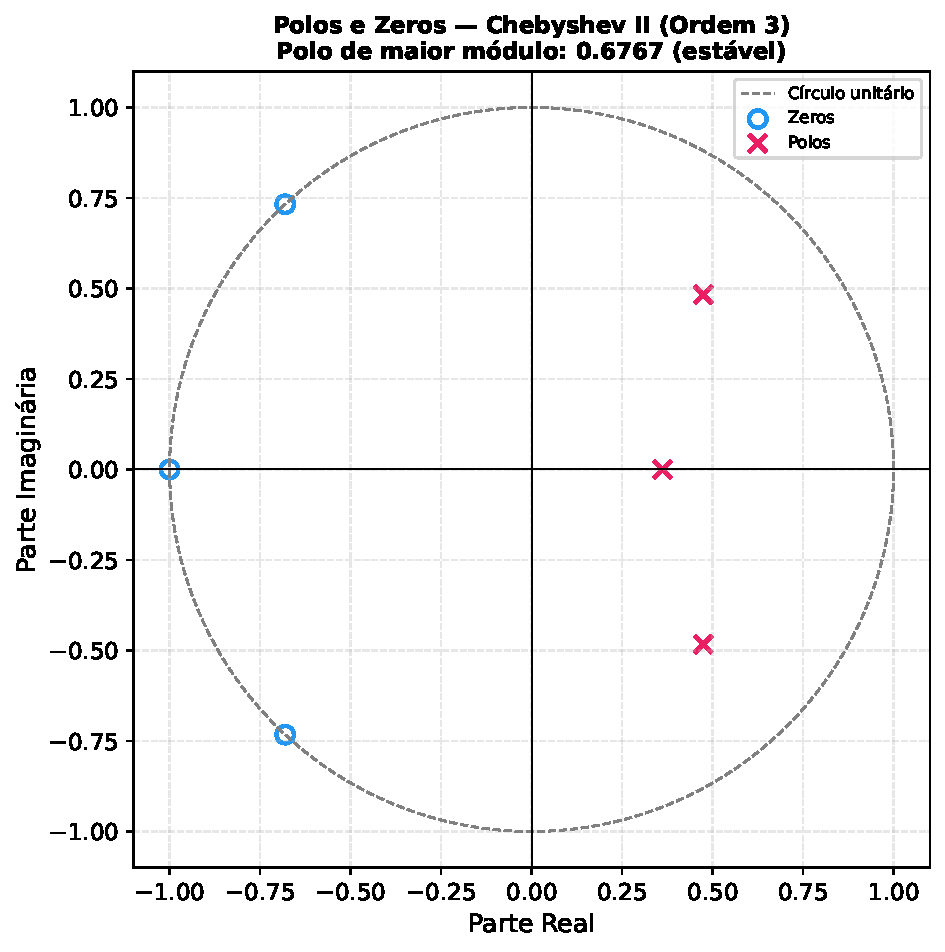
\includegraphics[width=0.78\columnwidth]{polos_zeros_b9.pdf}
\caption{Diagrama de polos e zeros do filtro Chebyshev~II de ordem~3.}
\label{fig:polos}
\end{figure}

O filtro Butterworth tem polos em $0{,}447 \pm j0{,}487$ e $0{,}349$, com módulo
máximo $|p|_{\max} = 0{,}661$; o Chebyshev~II, em $0{,}475 \pm j0{,}482$ e
$0{,}361$, com $|p|_{\max} = 0{,}677$. Como todos os polos têm módulo inferior à
unidade, ambos são estáveis no sentido BIBO (entrada limitada, saída limitada). A
Fig.~\ref{fig:polos} exibe o diagrama do Chebyshev~II: os três polos ficam bem no
interior do círculo unitário, enquanto um par de zeros se posiciona sobre o
círculo ($-0{,}681 \pm j0{,}733$), criando os \emph{notches} de transmissão
característicos dessa aproximação; os três zeros do Butterworth, em contraste,
coincidem em $z = -1$. A Fig.~\ref{fig:resposta} apresenta a resposta em
frequência (magnitude) dos quatro filtros, e a Fig.~\ref{fig:espectro}, o efeito
da filtragem sobre o espectro do sinal.

\begin{figure*}[t]
\centering
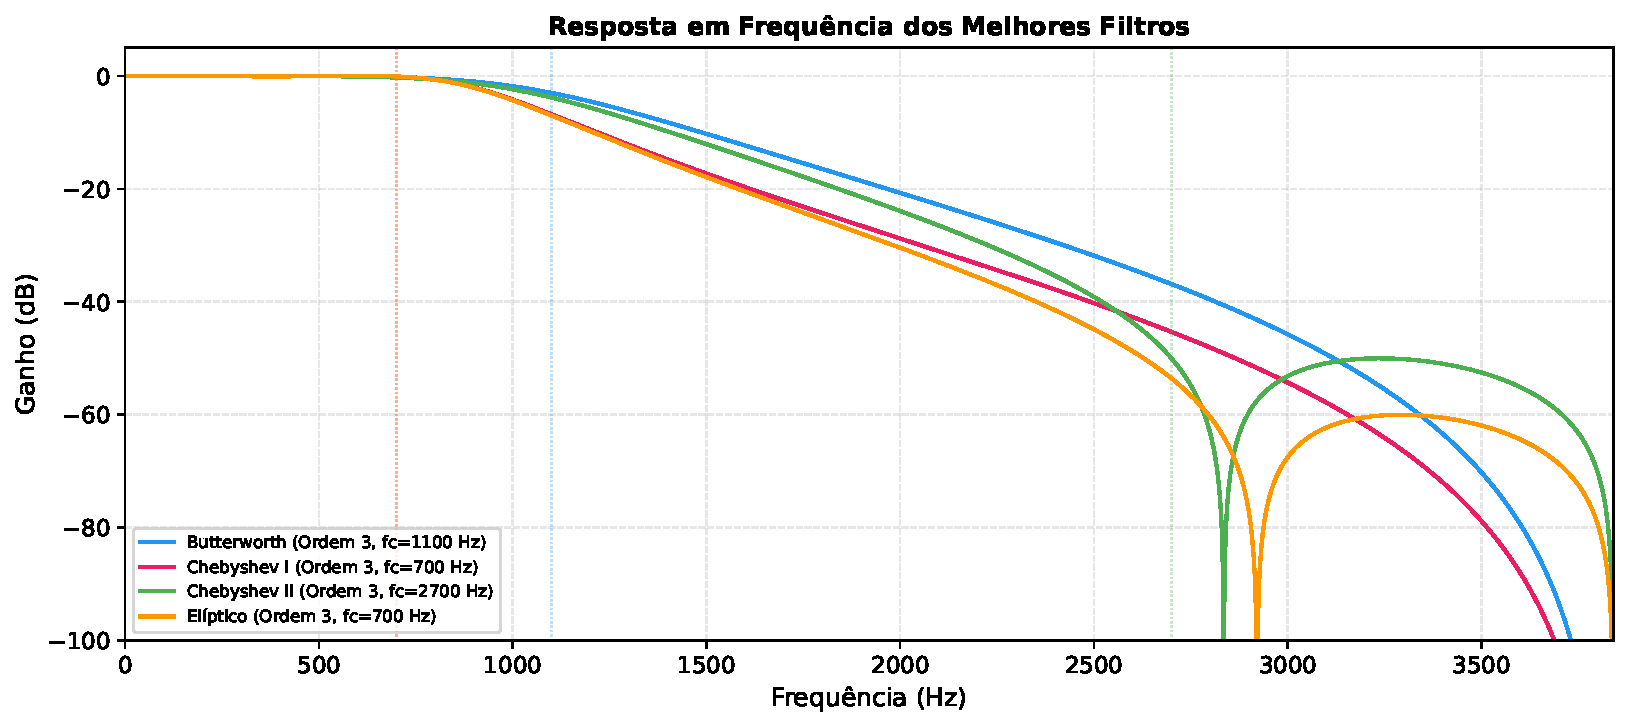
\includegraphics[width=0.85\textwidth]{resposta_frequencia_b9.pdf}
\caption{Resposta em frequência (magnitude) dos melhores filtros.}
\label{fig:resposta}
\end{figure*}

\begin{figure*}[t]
\centering
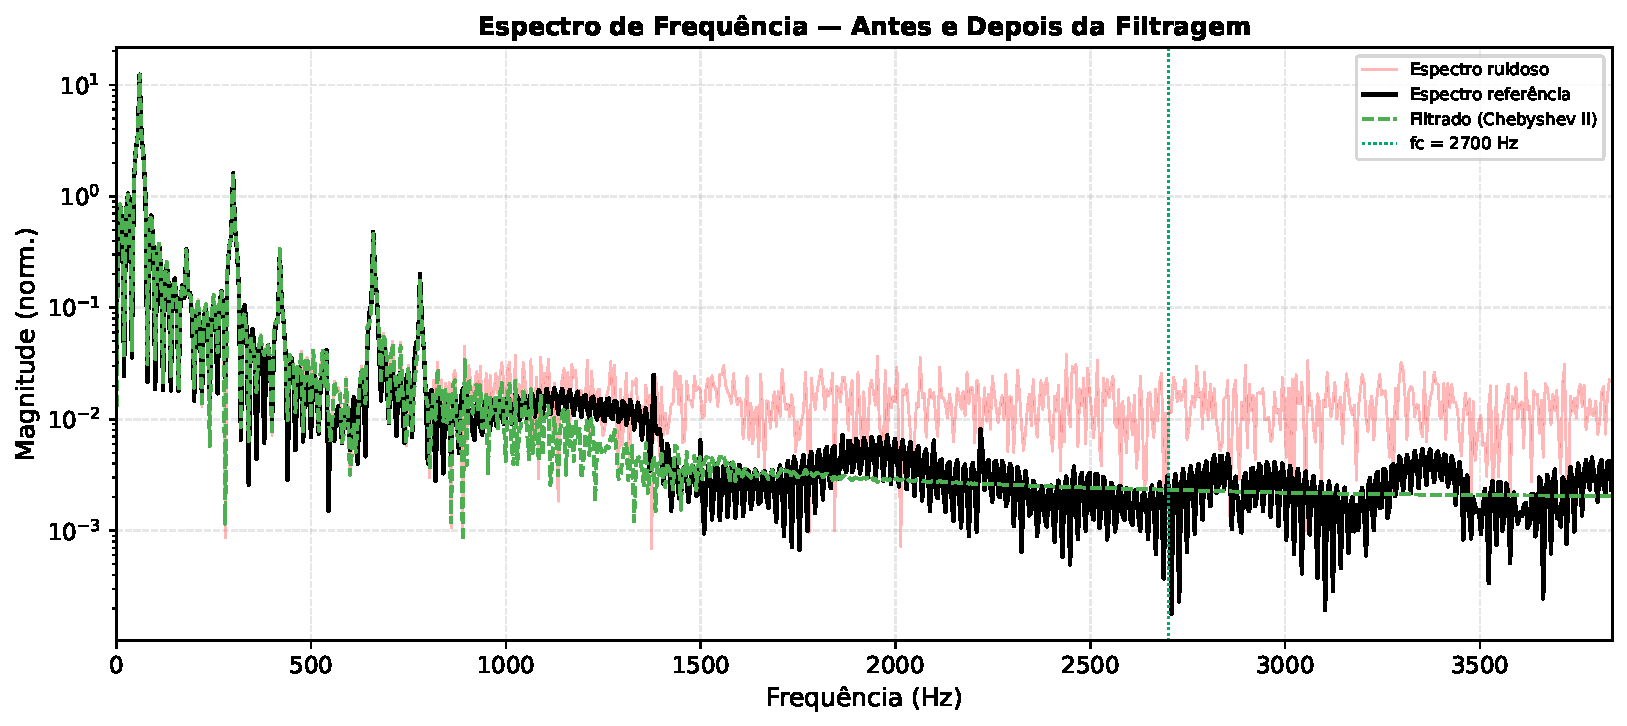
\includegraphics[width=0.85\textwidth]{espectro_fft_b9.pdf}
\caption{Espectro de magnitude (FFT) antes e depois da filtragem.}
\label{fig:espectro}
\end{figure*}

\begin{figure}[H]
\centering
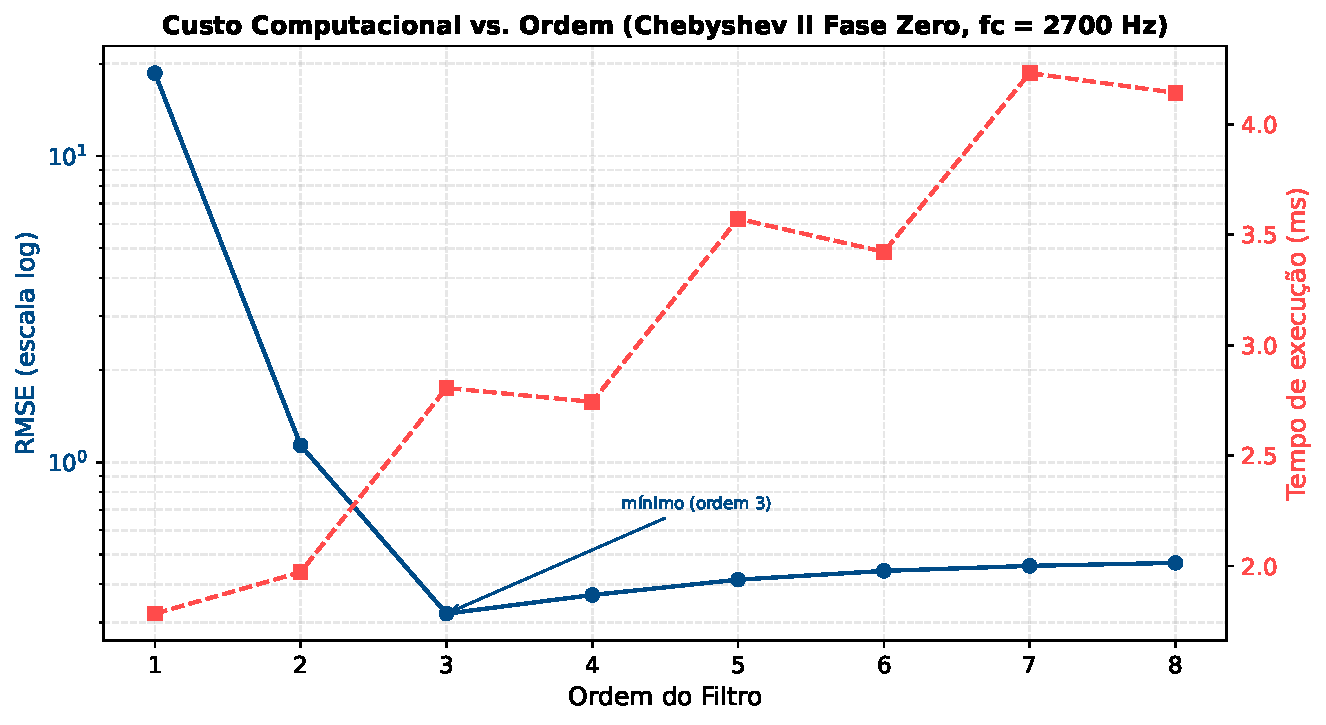
\includegraphics[width=\columnwidth]{custo_vs_ordem_b9.pdf}
\caption{RMSE e custo computacional em função da ordem do filtro.}
\label{fig:custo}
\end{figure}

Explique as parametrizações testadas para o algoritmo de processamento digital de sinais utilizado (se houver).

Demonstre, de preferência graficamente, as saídas do algoritmo de processamento digital de sinais utilizado. Ou traga valores tabelados. A Tabela~\ref{tab:results} exemplifica a tabulação de dados para apresentação de resultados.

\begin{table}[!h]
\renewcommand{\arraystretch}{1.2}
\caption{Dados tabulados.}
\label{tab:results}
\centering
\begin{tabular}{|c|ccccc|}
\hline
\multirow{2}{*}{\textbf{Zone}} & \multicolumn{5}{c|}{\textbf{MRE}} \\
 & \textbf{6-pulse} & \textbf{12-pulse} & \textbf{SFC} & \textbf{DC motor} & \textbf{TCR} \\
\hline
\textbf{1} & 15.2\% & 14.4\% & 32.2\% & 5.9\% & 35.2\% \\
\textbf{2} & 10.3\% & 12.0\%  & 7.1\% & 5.3\%  & 19.7\% \\
\textbf{3} & 0.6\% & 2.3\%  & 2.2\% & 1.3\%  & 0.5\% \\
\hline
\textbf{General} & 6.9\%  & 8.2\%  & 9.4\% & 3.7\%  & 14\% \\
\hline
\end{tabular}
\end{table}

Apresente e discuta os resultados finais de seu projeto. Pode usar gráficos e/ou tabelas. Entretanto, precisam ser devidamente explicados.


% !TEX root = ProjetoPDS.tex
\section{Conclusões}

A comparação entre as quatro aproximações deixou claro que o tipo de filtro
pesa tanto quanto a ordem ou a frequência de corte na qualidade do
resultado. Chebyshev~I e Elíptico convergiram, na busca em grade, para
ordem~1 com $f_c = \SI{600}{\hertz}$ -- um decaimento espectral lento demais
para separar o ruído sem comprometer o restante do sinal. Já o Butterworth
de ordem~3 melhorou esse cenário, mas, com $f_c = \SI{1100}{\hertz}$, acabou
atenuando parte das harmônicas de ordem $6k\pm1$ geradas pelas cargas não
lineares, o que se refletiu no RMSE.

O Chebyshev~II de ordem~3 e $f_c = \SI{2700}{\hertz}$ se destacou justamente
por combinar banda de passagem sem ripple, preservando a fundamental e as
harmônicas mais baixas, com zeros de transmissão na banda de rejeição, que
aceleram a queda do ganho logo após o corte. Essa combinação permitiu
remover o ruído de medição sem distorcer a informação harmônica, que é o que
de fato importa em uma análise de qualidade de energia.

O estudo do custo computacional em função da ordem reforça essa escolha: o
RMSE cai de forma acentuada até a ordem~3 e satura a partir daí, enquanto o
tempo de execução segue crescendo. Não há, portanto, ganho de precisão que
justifique usar uma ordem maior, apenas custo extra em uma aplicação que
poderia, em princípio, rodar em tempo real.

De forma geral, o trabalho mostra que projetar um filtro IIR não se resume a
escolher a aproximação com a transição mais rápida, mas sim a equilibrar
seletividade, fidelidade na banda de passagem e custo de implementação para
o sinal específico em questão.


\bibliographystyle{IEEEtran}
\bibliography{ref}

\appendix
% !TEX root = ProjetoPDS.tex
A implementação do código que projetou o filtro IIR computacional
foi feita com apoio de IA generativa, mais especificamente Claude e Gemini.
Primeiro, pedimos para que a ferramenta gerasse um código inicial
para o projeto do filtro; após testes de filtragem e verificação do
funcionamento, trabalhamos para incluir os diferentes tipos de filtros IIR e
simulamos ordens e frequências de corte diferentes, de modo a gerar os
gráficos de comparação. Em seguida, realizamos nossas análises e conclusões
com base nos resultados obtidos.

O código do projeto está disponível no repositório do GitHub, podendo ser
acessado através do link: \url{https://github.com/Aruanzin/Filtro-IIR}.
O repositório possui um README com instruções de como executar o código.


\end{document}
